% !TEX program = xelatex
\documentclass{beamer}
\usepackage{amsmath}
\usepackage{ctex}

\title{Feature mapping v.s. Deep Learning: \\Time Series Classification with/without physics}
\author{修格致, 邢潇月, 龚旭日}
\institute{Peking University}
\date{\today}

\begin{document}
    \maketitle    
\begin{frame}{Contents}
    \tableofcontents
\end{frame}

% Introduction
\section{Introduction}
\begin{frame}{Unfolding tasks}
    \begin{itemize}
        \item Feature engineering

    \begin{figure}
        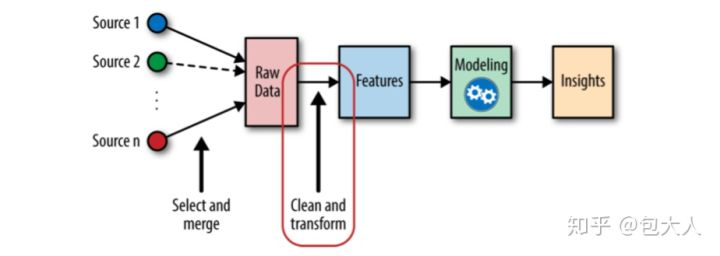
\includegraphics[width = 1\linewidth]{./pics/featuremap.jpg}
    \end{figure}
        \item 深度学习
    \end{itemize}

\end{frame}

\section{特征工程}

\begin{frame}{物理特征}
    \begin{itemize}
        \item 参数解译
        \begin{itemize}
            \item 加速度与重力加速度之间的关系?
        \item 重力加速度:
        \item 转动惯量的意义?
        \begin{itemize}
            \item 在哪里的人手机会转?
        \end{itemize}
    \end{itemize}
    \end{itemize}
\end{frame}

\begin{frame}{时间序列的特征选择}
    \begin{itemize}
        \item 全局特征
        \begin{itemize}
            \item 均值、方差、最值、谱
        \end{itemize} 
        \item 
    \end{itemize}
\end{frame}







\end{document}